%<<echo=FALSE>>=
%OLD <- options(width=90)
%@
%<<echo=FALSE>>=
%options(OLD)
%@

\documentclass{beamer}\usepackage[]{graphicx}\usepackage[]{color}
%% maxwidth is the original width if it is less than linewidth
%% otherwise use linewidth (to make sure the graphics do not exceed the margin)
\makeatletter
\def\maxwidth{ %
  \ifdim\Gin@nat@width>\linewidth
    \linewidth
  \else
    \Gin@nat@width
  \fi
}
\makeatother

\definecolor{fgcolor}{rgb}{0.102, 0.102, 0.102}
\newcommand{\hlnum}[1]{\textcolor[rgb]{0.2,0.2,0.2}{#1}}%
\newcommand{\hlstr}[1]{\textcolor[rgb]{0.2,0.2,0.2}{#1}}%
\newcommand{\hlcom}[1]{\textcolor[rgb]{0.302,0.302,0.302}{\textit{#1}}}%
\newcommand{\hlopt}[1]{\textcolor[rgb]{0.102,0.102,0.102}{#1}}%
\newcommand{\hlstd}[1]{\textcolor[rgb]{0.102,0.102,0.102}{#1}}%
\newcommand{\hlkwa}[1]{\textcolor[rgb]{0.102,0.102,0.102}{#1}}%
\newcommand{\hlkwb}[1]{\textcolor[rgb]{0.102,0.102,0.102}{#1}}%
\newcommand{\hlkwc}[1]{\textcolor[rgb]{0.2,0.2,0.2}{#1}}%
\newcommand{\hlkwd}[1]{\textcolor[rgb]{0.102,0.102,0.102}{\textbf{#1}}}%

\usepackage{framed}
\makeatletter
\newenvironment{kframe}{%
 \def\at@end@of@kframe{}%
 \ifinner\ifhmode%
  \def\at@end@of@kframe{\end{minipage}}%
  \begin{minipage}{\columnwidth}%
 \fi\fi%
 \def\FrameCommand##1{\hskip\@totalleftmargin \hskip-\fboxsep
 \colorbox{shadecolor}{##1}\hskip-\fboxsep
     % There is no \\@totalrightmargin, so:
     \hskip-\linewidth \hskip-\@totalleftmargin \hskip\columnwidth}%
 \MakeFramed {\advance\hsize-\width
   \@totalleftmargin\z@ \linewidth\hsize
   \@setminipage}}%
 {\par\unskip\endMakeFramed%
 \at@end@of@kframe}
\makeatother

\definecolor{shadecolor}{rgb}{.97, .97, .97}
\definecolor{messagecolor}{rgb}{0, 0, 0}
\definecolor{warningcolor}{rgb}{1, 0, 1}
\definecolor{errorcolor}{rgb}{1, 0, 0}
\newenvironment{knitrout}{}{} % an empty environment to be redefined in TeX

\usepackage{alltt}% regular slides (with pauses)
%\documentclass[handout]{beamer}% handout (no pauses)

%%%%%%%%%%%%%%%%%%%%%%%%%%%%%%%%%%%%%%%%%%%%%%%%%%%%%%%%%%%%%%%%%%%%%%%%%
%%%%%%% Change the lecture information here %%%%%%%%%%%%%%%%
\def\chapnum{Week \#2: Sampling from a Population (Sample Statistics have a Distribution)}
\title{Lecture 3: Probability}
\author{Kushal K Dey}
\date{}
%%%%%%%%%%%%%%%%%%%%%%%%%%%%%%%%%%%%%%%%%%%%%%%%%%%%%%%%%%%%%%%%%%%%%%%%%


\usepackage{enumerate}
\usepackage{amsmath, bbm}
\usepackage[misc]{ifsym} % for the dice symbol \Cube{}
\usepackage[latin1]{inputenc}
\usepackage{hyperref}

%\usepackage{comment}
%\usepackage{pstricks}
%\usepackage{graphicx}
%\usepackage{booktabs}
%\usepackage{pgfpages}
%\pgfpagesuselayout{2 on 1}[a4paper,border shrink=3mm]
%\pgfpagesuselayout{4 on 1}[a4paper,landscape,border shrink=3mm

\usepackage{setspace}
\ifdefined\knitrout
  \renewenvironment{knitrout}{\begin{spacing}{0.75}\begin{tiny}}{\end{tiny}\end{spacing}}
\else
\fi

%%%%%%%%%%%%%%% Defined Shortcuts (macros) %%%%%%%%%%%%%
% parameters and statistics
\newcommand{\xbar}{\overline{x}}
\newcommand{\Xbar}{\overline{X}}
\newcommand{\ybar}{\overline{y}}
\newcommand{\Ybar}{\overline{Y}}
\newcommand{\dbar}{\overline{d}}
\newcommand{\Dbar}{\overline{D}}
\newcommand{\zbar}{\overline{z}}
\newcommand{\Zbar}{\overline{Z}}
\newcommand{\ehat}{\widehat{\epsilon}}
\newcommand{\yhat}{\widehat{y}}
\newcommand{\Yhat}{\widehat{Y}}
\newcommand{\betaa}{{\beta_0}}
\newcommand{\betab}{{\beta_1}}
\newcommand{\betac}{{\beta_2}}
\newcommand{\betad}{{\beta_3}}
\newcommand{\BETA}{{\boldsymbol\beta}}
\newcommand{\betahata}{\widehat{\beta_0}}
\newcommand{\betahatb}{\widehat{\beta_1}}
\newcommand{\betahatc}{\widehat{\beta_2}}
\newcommand{\betahatd}{\widehat{\beta_3}}
\newcommand{\bhat}{\widehat{b}}
\newcommand{\btilde}{\widetilde{b}}
\newcommand{\ahat}{\widehat{a}}
\newcommand{\atilde}{\widetilde{a}}
\newcommand{\rss}{\mathit{SSE}}
\newcommand{\sigmahat}{\widehat{\sigma}}
\newcommand{\betahat}{\widehat{\beta}}
\newcommand{\thetahat}{\widehat{\theta}}
\newcommand{\phat}{\widehat{p}}
\newcommand{\pihat}{\widehat{\pi}}
\newcommand{\muhat}{\widehat{\mu}}
% real numbers and integers
\newcommand{\reals}{\mathbbm{R}}
\newcommand{\integers}{\mathbbm{N}}
%distributions
\newcommand{\normal}{\textsf{Norm}}
\newcommand{\Bin}{\textsf{Binom}}
\newcommand{\Uni}{\textsf{Unif}}
\newcommand{\Poisson}{\textsf{Pois}}
\newcommand{\Exp}{\textsf{Exp}}
\newcommand{\Beta}{\textsf{Beta}}
\newcommand{\iid}{\stackrel{\mathrm{iid}}{\sim}}
% probability and expected value
\newcommand{\rv}{r.v.\ }
\newcommand{\prob}{{\rm P}}
\newcommand{\mean}{\mathrm{E}}
\newcommand{\var}{\mathrm{Var}}
\newcommand{\Var}{\mathrm{Var}}
\newcommand{\cov}{\mathrm{Cov}}
\newcommand{\corr}{\mathop{\mathrm{Corr}}}
% measures of spread
\newcommand{\IQR}{\textit{IQR}}
\newcommand{\SAD}{\textit{SAD}}
\newcommand{\MAD}{\textit{MAD}}
\newcommand{\SSD}{\textit{SSD}}
\newcommand{\MSD}{\textit{MSD}}
\newcommand{\RMSD}{\textit{RMSD}}
\newcommand{\MSE}{\textit{MSE}}
\newcommand{\MSR}{\textit{MSR}}
% formatting code and such
\providecommand{\variable}[1]{}
\renewcommand{\variable}[1]{{\color{green!50!black}\texttt{#1}}}
\providecommand{\function}[1]{}
\renewcommand{\function}[1]{{\color{purple!75!blue}\texttt{\StrSubstitute{#1}{()}{}()}}}
\providecommand{\option}[1]{}
\renewcommand{\option}[1]{{\color{brown!80!black}\texttt{#1}}}
\providecommand{\pkg}[1]{}
\renewcommand{\pkg}[1]{{\color{red!80!black}\texttt{#1}}}
\providecommand{\code}[1]{}
\renewcommand{\code}[1]{{\color{blue!80!black}\texttt{#1}}}

%%%%%%%%%
% Changed by Kushal K Dey, University of Chicago
%\providecommand{\file}[1]{}
%\renewcommand{\file}[1]{{\tt #1}}
\providecommand{\file}[1]{}
\renewcommand{\file}[1]{{\color{orange!80!black}\texttt{#1}}}
%\providecommand{\dataframe}[1]{}
%\renewcommand{\dataframe}[1]{{\color{blue!80!black}\texttt{#1}}}
\providecommand{\dataframe}[1]{}
\renewcommand{\dataframe}[1]{{\color{cyan!80!black}\texttt{#1}}}
%%%%%%%%%

% other
\def\Sum{\sum\nolimits}
\def\b#1{\fboxsep=0pt\colorbox{black}{\color{white}\Cube{#1}}}
\def\w#1{\Cube{#1}}
%%%%%%%%%%%% End of shortcuts (macros) ##############

%%%%%%%%% One way to hide answers until you want to show them %%%%%%%%%
\def\Hide#1#2{\ul{~~~\onslide<#1>{\alert{#2}}~~~}}
\def\hide#1#2{\ul{~~\onslide<#1>{\alert{#2}}~~}}
\def\hid#1#2{\onslide<#1>{\alert{#2}}}
% Choose the color of answers here too
\setbeamercolor{alerted text}{fg=darkgray}
%\setbeamercolor{alerted text}{fg=black}

%------Centered Page Number Setup ------
\defbeamertemplate{footline}{centered page number}
{%
  \hspace*{\fill}%
  %\usebeamercolor[fg]{page number in head/foot}%
  %\usebeamerfont{page number in head/foot}%
  \tiny \chapnum: Page \insertframenumber\, of \inserttotalframenumber%
  \hspace*{\fill}\vskip2pt%
}
%\setbeamertemplate{footline}{\hfill\insertframenumber/\inserttotalframenumber}
\setbeamertemplate{footline}[centered page number]
%--------------------------------

%\usetheme{Copenhagen}
\setbeamertemplate{navigation symbols}{}
\usepackage[english]{babel}
\def\ul{\underline}
\linespread{1.1}
% or whatever



%\parskip=0pt
\IfFileExists{upquote.sty}{\usepackage{upquote}}{}
\begin{document}%large

%<<setup, include=FALSE, cache=FALSE>>=
%options(replace.assign=TRUE,width=90, digits=4)
%opts_chunk$set(fig.path='figure/graphics-', cache.path='cache/graphics-', fig.align='center', fig.width=8, fig.height=5.5, fig.show='as.is', out.width='0.9\\linewidth', cache=FALSE, par=TRUE, size = 'tiny', tidy=TRUE, cache.extra=rand_seed)
%knit_hooks$set(par=function(before, options, envir){
%if (before && options$fig.show!='none') par(mar=c(4,4,.1,.1),cex.lab=.95,cex.axis=.9,mgp=c(2,.7,0),tcl=-.3)
%}, document = function(x) {
%  gsub('\\\\(begin|end)\\{kframe\\}', '', x)
%}, crop=hook_pdfcrop)
%@
%<<setup2, include=FALSE, cache=FALSE>>=
%knit_theme$set("print")
%@


%%%%%%%%%%%%%%%%%%%%%%%%%%%%%%%%%%%%%%%%%%%%%%%%%%%%%%%%%%%%%%%%%%%%%%%%%
%%%%%%%%%%%%%%%%%%%%%%%%%%%%%%%%%%%%%%%%%%%%%%%%%%%%%%%%%%%%%%%%%%%%%%%%%
%%%%%% End of suggested definitions and packages %%%%%%%%%%%%

%------------------------------------------------------------------
%------------------------------------------------------------------

%%%%%%%%%% Title frame (optional) %%%%%%%%%%%%%
\begin{frame}{}
\maketitle
\end{frame}
%%%%%%%%%%%%%%%%%%%%%%%%%%%%%%%%%%%%%%%%%%%%%%%

%%%%%%%%%%%%%% Begin slides here %%%%%%%%%%%%%%

%%%%%%%%%%%%%%%%%%%%%%%%%%%%%%%%%%%%%%%%%%%%%%%%%%%%%%%%%%%%
\begin{frame}[fragile]{Toss a coin \;\;}
%%%%%%%%%%%%%%%%%%%%%%%%%%%%%%%%%%%%%%%%%%%%%%%%%%%%%%%%%%%%

\begin{knitrout}\small
\definecolor{shadecolor}{rgb}{1, 1, 1}\color{fgcolor}\begin{kframe}
\begin{alltt}
\hlstd{TossCoin} \hlkwb{<-} \hlkwa{function}\hlstd{(}\hlkwc{n}\hlstd{=}\hlnum{1}\hlstd{)\{}
    \hlkwd{return}\hlstd{(}\hlkwd{replicate}\hlstd{(n,} \hlkwd{sample}\hlstd{(}\hlkwd{c}\hlstd{(}\hlstr{"H"}\hlstd{,}\hlstr{"T"}\hlstd{),}\hlnum{1}\hlstd{)))}
\hlstd{\}}
\hlkwd{TossCoin}\hlstd{(}\hlnum{1}\hlstd{)}
\end{alltt}
\begin{verbatim}
[1] "T"
\end{verbatim}
\begin{alltt}
\hlkwd{TossCoin}\hlstd{(}\hlkwc{n}\hlstd{=}\hlnum{2}\hlstd{)}
\end{alltt}
\begin{verbatim}
[1] "T" "H"
\end{verbatim}
\begin{alltt}
\hlkwd{TossCoin}\hlstd{(}\hlkwc{n}\hlstd{=}\hlnum{10}\hlstd{)}
\end{alltt}
\begin{verbatim}
 [1] "H" "H" "T" "H" "T" "T" "T" "T" "H" "H"
\end{verbatim}
\end{kframe}
\end{knitrout}

\end{frame}
%%%%%%%%%%%%%%%%%%%%%%%%%%%%%%%%%%%%%%%%%%%%%%%%%%%%%%%%%%%%

%%%%%%%%%%%%%%%%%%%%%%%%%%%%%%%%%%%%%%%%%%%%%%%%%%%%%%%%%%%%
\begin{frame}[fragile]{Experimental States \;\;}
%%%%%%%%%%%%%%%%%%%%%%%%%%%%%%%%%%%%%%%%%%%%%%%%%%%%%%%%%%%%

All possible states of an experiment.

1 toss of coin: $\left \{ H, T  \right \}$ \pause \newline

2 tosses : $\left \{H, H \right \}, \left \{H, T \right \}, \left \{T, H \right \},
            \left \{T, T \right \}$ \pause \newline

10 tosses: $\left\{x_{1}x_{2} \cdots x_{n} : x_{i} \in \{H,T \} \right \}$

\end{frame}
%%%%%%%%%%%%%%%%%%%%%%%%%%%%%%%%%%%%%%%%%%%%%%%%%%%%%%%%%%%%

%%%%%%%%%%%%%%%%%%%%%%%%%%%%%%%%%%%%%%%%%%%%%%%%%%%%%%%%%%%%
\begin{frame}[fragile]{Random Variable \;\;}
%%%%%%%%%%%%%%%%%%%%%%%%%%%%%%%%%%%%%%%%%%%%%%%%%%%%%%%%%%%%

A function that associates a unique numerical value with every outcome of an experiment. \pause \newline

For example, associate $1$ with H and $0$ with T in 1 coin toss experiment. \pause \newline

The value of the random variable will vary from trial to trial as the experiment is repeated. \pause \newline

Ex: A coin is tossed 2 times. The random variable X is the number of tails that are noted.

\begin{tabular}{|c|c|}
\hline
state & X \\ \hline
HH & 0 \\ \hline
HT & 1 \\ \hline
TH & 1 \\ \hline
TT & 2 \\ \hline
\end{tabular}

\end{frame}
%%%%%%%%%%%%%%%%%%%%%%%%%%%%%%%%%%%%%%%%%%%%%%%%%%%%%%%%%%%%


%%%%%%%%%%%%%%%%%%%%%%%%%%%%%%%%%%%%%%%%%%%%%%%%%%%%%%%%%%%%
\begin{frame}[fragile]{Events \;\;}
%%%%%%%%%%%%%%%%%%%%%%%%%%%%%%%%%%%%%%%%%%%%%%%%%%%%%%%%%%%%

Are all the states of an experiment equally likely? \pause \newline

What if a coin is biased to come up heads $80 \%$ times? \pause \newline

Events: Sets of outcomes of the experiment \pause \newline

 $X=1$ is an event, comprises of two outcomes $\{HT, TH \}$ \pause ]\newline

 $X=2$ is also an event, comprises of $\{ HH \}$. \pause \newline

 $X=0$ is also an event, comprises of $\{ TT \}$.

\end{frame}
%%%%%%%%%%%%%%%%%%%%%%%%%%%%%%%%%%%%%%%%%%%%%%%%%%%%%%%%%%%%

%%%%%%%%%%%%%%%%%%%%%%%%%%%%%%%%%%%%%%%%%%%%%%%%%%%%%%%%%%%%
\begin{frame}[fragile]{Events  \;\;}
%%%%%%%%%%%%%%%%%%%%%%%%%%%%%%%%%%%%%%%%%%%%%%%%%%%%%%%%%%%%

Take another example. Let X be a random variable that takes 1 if there is
at least one head. \pause \newline

\begin{tabular}{|c|c|}
\hline
state & X \\ \hline
HH & 1 \\ \hline
HT & 1 \\ \hline
TH & 1 \\ \hline
TT & 0 \\ \hline
\end{tabular}

Then  $X=1$ is an event, comprises of two outcomes $\{HH, HT, TH \}$ \pause \newline

$X=0$ is also an event, comprises of $\{ TT \}$.

\end{frame}
%%%%%%%%%%%%%%%%%%%%%%%%%%%%%%%%%%%%%%%%%%%%%%%%%%%%%%%%%%%%

%%%%%%%%%%%%%%%%%%%%%%%%%%%%%%%%%%%%%%%%%%%%%%%%%%%%%%%%%%%%
\begin{frame}[fragile]{Probability  \;\;}
%%%%%%%%%%%%%%%%%%%%%%%%%%%%%%%%%%%%%%%%%%%%%%%%%%%%%%%%%%%%

Take any experiment (say 2 independent tosses of a coin).  \pause \newline

In one experiment, there may be many states (4 in this case- HH, HT, TH and TT) but remember, you observe only one. \pause \newline

Repeat the experiment many many times (as many as you can imagine- may be $10^7$). \pause \newline

The proportion of times you observe each experimental state after all these many repititions gives you the probability of that state.

\end{frame}
%%%%%%%%%%%%%%%%%%%%%%%%%%%%%%%%%%%%%%%%%%%%%%%%%%%%%%%%%%%%

%%%%%%%%%%%%%%%%%%%%%%%%%%%%%%%%%%%%%%%%%%%%%%%%%%%%%%%%%%%%
\begin{frame}[fragile]{Example of Probability  \;\;}
%%%%%%%%%%%%%%%%%%%%%%%%%%%%%%%%%%%%%%%%%%%%%%%%%%%%%%%%%%%%

We cite an example of how to measure probability for one coin toss with states
H and T.

\url{http://digitalfirst.bfwpub.com/stats_applet/stats_applet_10_prob.html}
\pause \newline

Cases: Coin fair and unfair!! \pause \newline

Question : What is the \emph{probability} of Heads in a coin toss? \pause \newline

Reframe the question: What is the proportion of times you would expect to see
Heads if you tossed the coin many many times? \pause \newline

\end{frame}
%%%%%%%%%%%%%%%%%%%%%%%%%%%%%%%%%%%%%%%%%%%%%%%%%%%%%%%%%%%%

%%%%%%%%%%%%%%%%%%%%%%%%%%%%%%%%%%%%%%%%%%%%%%%%%%%%%%%%%%%%
\begin{frame}[fragile]{Probability  Table \;\;}
%%%%%%%%%%%%%%%%%%%%%%%%%%%%%%%%%%%%%%%%%%%%%%%%%%%%%%%%%%%%

For a fair toss of coin, we saw

\begin{tabular}{|c|c|}
\hline
state & Prob \\ \hline
H & Pr(H) = 0.5\\ \hline
T & Pr(T) = 0.5 \\ \hline
\end{tabular} \pause \newline

Let $X$ be 1 if state is H and 0 if T. \pause \newline

\begin{tabular}{|c|c|}
\hline
X & Prob \\ \hline
1 & Pr(X=1) := Pr(H) = 0.5\\ \hline
0 & Pr(X=0) := Pr(T) = 0.5 \\ \hline
\end{tabular}

\end{frame}
%%%%%%%%%%%%%%%%%%%%%%%%%%%%%%%%%%%%%%%%%%%%%%%%%%%%%%%%%%%%

%%%%%%%%%%%%%%%%%%%%%%%%%%%%%%%%%%%%%%%%%%%%%%%%%%%%%%%%%%%%
\begin{frame}[fragile]{Probability  of an Event \;\;}
%%%%%%%%%%%%%%%%%%%%%%%%%%%%%%%%%%%%%%%%%%%%%%%%%%%%%%%%%%%%

\emph{Probability of an event} is the sum of probability of all states making up the event. \pause \newline

For two independent tosses of a fair coin, the probability table on states \pause \newline

\begin{tabular}{|c|c|}
\hline
state & Prob \\ \hline
HH & Pr(HH) = Pr(H in toss 1) * Pr(H in toss 2) = 0.25\\ \hline
HT & Pr(HT) = Pr(H in toss 1) * Pr(T in toss 2) = 0.25 \\ \hline
TH & Pr(TH) = Pr(T in toss 1) * Pr(H in toss 2) = 0.25\\ \hline
TT & Pr(HT) = Pr(T in toss 1) * Pr(T in toss 2) = 0.25 \\ \hline
\end{tabular} \pause \newline

\end{frame}
%%%%%%%%%%%%%%%%%%%%%%%%%%%%%%%%%%%%%%%%%%%%%%%%%%%%%%%%%%%%

%%%%%%%%%%%%%%%%%%%%%%%%%%%%%%%%%%%%%%%%%%%%%%%%%%%%%%%%%%%%
\begin{frame}[fragile]{Probability  of an Event \;\;}
%%%%%%%%%%%%%%%%%%%%%%%%%%%%%%%%%%%%%%%%%%%%%%%%%%%%%%%%%%%%

Let X be 1 if we observe at least one H in two coin tosses. \pause \newline

Then the probability table for the random variable X. \newline

\begin{tabular}{|c|c|c|}
\hline
X & states & Prob \\ \hline
0 & TT & Pr(X=0) = Pr(TT) = 0.25 \\ \hline
1 & \{ HH, HT, TH \} & Pr(X=1) = Pr(HH) + Pr(HT) + Pr(TH) = 0.75 \\ \hline
\end{tabular} \newline \newline

Note that the sum of the probabilities for any probability table would be 1 (sum across all possible states).

\end{frame}
%%%%%%%%%%%%%%%%%%%%%%%%%%%%%%%%%%%%%%%%%%%%%%%%%%%%%%%%%%%%


%%%%%%%%%%%%%%%%%%%%%%%%%%%%%%%%%%%%%%%%%%%%%%%%%%%%%%%%%%%%
\begin{frame}[fragile]{Probability  of an Event \;\;}
%%%%%%%%%%%%%%%%%%%%%%%%%%%%%%%%%%%%%%%%%%%%%%%%%%%%%%%%%%%%

Let X be number of Ts observed in two tosses of a coin \pause \newline

Then the probability table for the random variable X. \newline

\begin{tabular}{|c|c|c|}
\hline
X & states & Prob \\ \hline
0 & HH & Pr(X=0) = Pr(HH) = 0.25 \\ \hline
1 & \{ HT, TH \} & Pr(X=1) = Pr(HT) + Pr(TH) = 0.50 \\ \hline
2 & TT & Pr(X=2) = Pr(TT) = 0.25 \\ \hline
\end{tabular} \newline \newline

Note that the sum of the probabilities for any probability table would be 1 (sum across all possible states).

\end{frame}
%%%%%%%%%%%%%%%%%%%%%%%%%%%%%%%%%%%%%%%%%%%%%%%%%%%%%%%%%%%%

%%%%%%%%%%%%%%%%%%%%%%%%%%%%%%%%%%%%%%%%%%%%%%%%%%%%%%%%%%%%
\begin{frame}[fragile]{Why do we need Random variables? \;\;}
%%%%%%%%%%%%%%%%%%%%%%%%%%%%%%%%%%%%%%%%%%%%%%%%%%%%%%%%%%%%

When we can define probability in terms of states and events, why do we need random variable X? \pause \newline

\emph{It is easier to interpret the experiment through numbers and bunch of symbols}.

What type of interpreting? \pause \newline

Measures of central tendency and spread

\end{frame}
%%%%%%%%%%%%%%%%%%%%%%%%%%%%%%%%%%%%%%%%%%%%%%%%%%%%%%%%%%%%

%%%%%%%%%%%%%%%%%%%%%%%%%%%%%%%%%%%%%%%%%%%%%%%%%%%%%%%%%%%%
\begin{frame}[fragile]{Probability distribution of random variable \;\;}
%%%%%%%%%%%%%%%%%%%%%%%%%%%%%%%%%%%%%%%%%%%%%%%%%%%%%%%%%%%%

Suppose $X$ is a random variable that takes values $x_{1}, x_{2}, \cdots. x_{n}$
and let us define the probability

$$ p(x_{i}) = Pr(X=x_{i}) $$

Then we have

$$ 0 \leq p(x_{i}) \leq 1 $$

$$ \sum_{i=1}^{n} p(x_{i}) = 1 $$

Cumulative probability

$$ F(x) = Pr(X \leq x) = \sum_{x_{i} \leq x} p(x_{i}) $$

\end{frame}
%%%%%%%%%%%%%%%%%%%%%%%%%%%%%%%%%%%%%%%%%%%%%%%%%%%%%%%%%%%%


%%%%%%%%%%%%%%%%%%%%%%%%%%%%%%%%%%%%%%%%%%%%%%%%%%%%%%%%%%%%
\begin{frame}[fragile]{Expectation of random variable \;\;}
%%%%%%%%%%%%%%%%%%%%%%%%%%%%%%%%%%%%%%%%%%%%%%%%%%%%%%%%%%%%

If X is a discrete random variable with possible values $x_1, x_2, x_3, ..., x_n$

$$ E(X) : = \sum_{i=1}^{n} x_{i} Pr(X=x_{i})  $$

For one coin toss, let X be 1 if H and 0 if T.

$$ E(X) = 0. Pr(X=0) + 1. Pr(X=1) = 0.5 $$

If X is number of Ts in 2 independent tosses of a coin

$$ E(X) = 0. Pr(X=0) + 1. Pr(X=1) + 2. Pr(X=2) = 0 + 0.5 + 2*0.25 = 1 $$

If I am asked to choose ONE value of the variable X, this is the value we may want to choose.

\end{frame}
%%%%%%%%%%%%%%%%%%%%%%%%%%%%%%%%%%%%%%%%%%%%%%%%%%%%%%%%%%%%


%%%%%%%%%%%%%%%%%%%%%%%%%%%%%%%%%%%%%%%%%%%%%%%%%%%%%%%%%%%%
\begin{frame}[fragile]{Expectation and $\bar{x}$ \;\;}
%%%%%%%%%%%%%%%%%%%%%%%%%%%%%%%%%%%%%%%%%%%%%%%%%%%%%%%%%%%%

We saw that if we observe values $x_1, x_2, \cdots, x_{n}$ with frequencies $f_{1}, f_{2}, \cdots, f_{n}$, then

$$ \bar{x} := \frac{1}{n} \sum_{i=1}^{n} x_i f_i = \frac{1}{n} \sum_{i=1}^{n} x_{i} \left ( \frac{f_{i}}{n} \right ) $$

Now we can argue that as $n \rightarrow \infty$, $\frac{f_i}{n} \approx Pr(X=x_{i})$,
then we get the expectation

$$ E(X) = \sum_{i=1}^{n} x_{i} Pr (X= x_{i}) $$

\end{frame}
%%%%%%%%%%%%%%%%%%%%%%%%%%%%%%%%%%%%%%%%%%%%%%%%%%%%%%%%%%%%

%%%%%%%%%%%%%%%%%%%%%%%%%%%%%%%%%%%%%%%%%%%%%%%%%%%%%%%%%%%%
\begin{frame}[fragile]{Law of Large Numbers \;\;}
%%%%%%%%%%%%%%%%%%%%%%%%%%%%%%%%%%%%%%%%%%%%%%%%%%%%%%%%%%%%

Seems like as $n$ becomes larger, the sample average $\bar{X}_{n}$ becomes closer and closer to the population average $\mu= E(X)$. \pause \newline

Can we mathematically formulate it.

$$ Pr ( \left | \bar{X}_{n} - \mu \right | > \delta) \rightarrow 0 $$

for any $\delta > 0 $.

\end{frame}
%%%%%%%%%%%%%%%%%%%%%%%%%%%%%%%%%%%%%%%%%%%%%%%%%%%%%%%%%%%%

%%%%%%%%%%%%%%%%%%%%%%%%%%%%%%%%%%%%%%%%%%%%%%%%%%%%%%%%%%%%
\begin{frame}[fragile]{Law of Large Numbers \;\;}
%%%%%%%%%%%%%%%%%%%%%%%%%%%%%%%%%%%%%%%%%%%%%%%%%%%%%%%%%%%%

Lets go back to the applet:

\url{http://digitalfirst.bfwpub.com/stats_applet/stats_applet_10_prob.html}
\pause \newline

By Law of Large Numbers (LLN), if you toss the coin many times, say 100, you should expect to get closely similar number of heads and tails.  \pause \newline

If you tossed it many more times than 100, say 10,000, you would expect to
get even closer to a 1:1 ratio of heads and tails (closer and closer
to $50\%$ heads and $50 \%$ tails). \pause \newline

The more times you repeat the experiment, the closer you should get to the true probability (which remember is proportion for infinite many trials).

\end{frame}
%%%%%%%%%%%%%%%%%%%%%%%%%%%%%%%%%%%%%%%%%%%%%%%%%%%%%%%%%%%%


%%%%%%%%%%%%%%%%%%%%%%%%%%%%%%%%%%%%%%%%%%%%%%%%%%%%%%%%%%%%
\begin{frame}[fragile]{Variance \;\;}
%%%%%%%%%%%%%%%%%%%%%%%%%%%%%%%%%%%%%%%%%%%%%%%%%%%%%%%%%%%%

\emph{Variance of a random variable} is a non-negative number which gives an idea of how widely spread the values of the random variable are likely to be; the larger the variance, the more scattered the observations on average. \pause \newline

Define it as

\begin{align}
Var(X) & : = \sum_{i=1}^{n} (x_{i} - E(X))^2 Pr(X=x_{i})  \\
          & = E(X - E(X))^2 \\
          & = E(X^2) - E(X)^2 \\
          & = \sum_{i=1}^{n} x^2_{i} Pr(X=x_{i}) - \left (\sum_{i=1}^{n} x_{i} Pr (X= x_{i}) \right)^2 \\
\end{align}

\end{frame}
%%%%%%%%%%%%%%%%%%%%%%%%%%%%%%%%%%%%%%%%%%%%%%%%%%%%%%%%%%%%

%%%%%%%%%%%%%%%%%%%%%%%%%%%%%%%%%%%%%%%%%%%%%%%%%%%%%%%%%%%%
\begin{frame}[fragile]{Chebyshev Inequality \;\;}
%%%%%%%%%%%%%%%%%%%%%%%%%%%%%%%%%%%%%%%%%%%%%%%%%%%%%%%%%%%%

\emph{General Chebyshev Inequality:}  For any random variable $X$, for any fixed $\epsilon>0$

$$ Pr [ g(X) \geq \epsilon ] \leq \frac { E (g(X)) }{\epsilon} $$

\emph{Chebyshev Inequality:}

$$ Pr [ \left | \bar{X}_{n} - \mu \right | \geq \epsilon ] \leq \frac{E(\bar{X}_{n} - \mu)^2}{\epsilon^2}  $$

\end{frame}
%%%%%%%%%%%%%%%%%%%%%%%%%%%%%%%%%%%%%%%%%%%%%%%%%%%%%%%%%%%%

%%%%%%%%%%%%%%%%%%%%%%%%%%%%%%%%%%%%%%%%%%%%%%%%%%%%%%%%%%%%
\begin{frame}[fragile]{Our first Probability Distribution \;\;}
%%%%%%%%%%%%%%%%%%%%%%%%%%%%%%%%%%%%%%%%%%%%%%%%%%%%%%%%%%%%

Let $X$ be a random variable taking values 0 and 1 for T and H in a coin toss experiment. \pause \newline

\begin{align}
X & = 1 \hspace{0.5 cm}  \;\; prob \;\; p \\
  & = 0 \hspace{0.5 cm}  \;\;prob \;\; (1-p) \\
\end{align}

where $p$ is the probability of head (0.5 in fair coin toss case).\pause \newline

This distribution is called a \textbf{Bernoulli distribution} and we term
$ X \sim Ber(p) $

$$ E(X) = p \hspace{0.5 cm} var(X) = E(X^2) - E(X)^2 = p - p^2 = p(1-p) $$

\end{frame}
%%%%%%%%%%%%%%%%%%%%%%%%%%%%%%%%%%%%%%%%%%%%%%%%%%%%%%%%%%%%


%%%%%%%%%%%%%%%%%%%%%%%%%%%%%%%%%%%%%%%%%%%%%%%%%%%%%%%%%%%%
\begin{frame}[fragile]{Bernoulli distribution graph \;\;}
%%%%%%%%%%%%%%%%%%%%%%%%%%%%%%%%%%%%%%%%%%%%%%%%%%%%%%%%%%%%


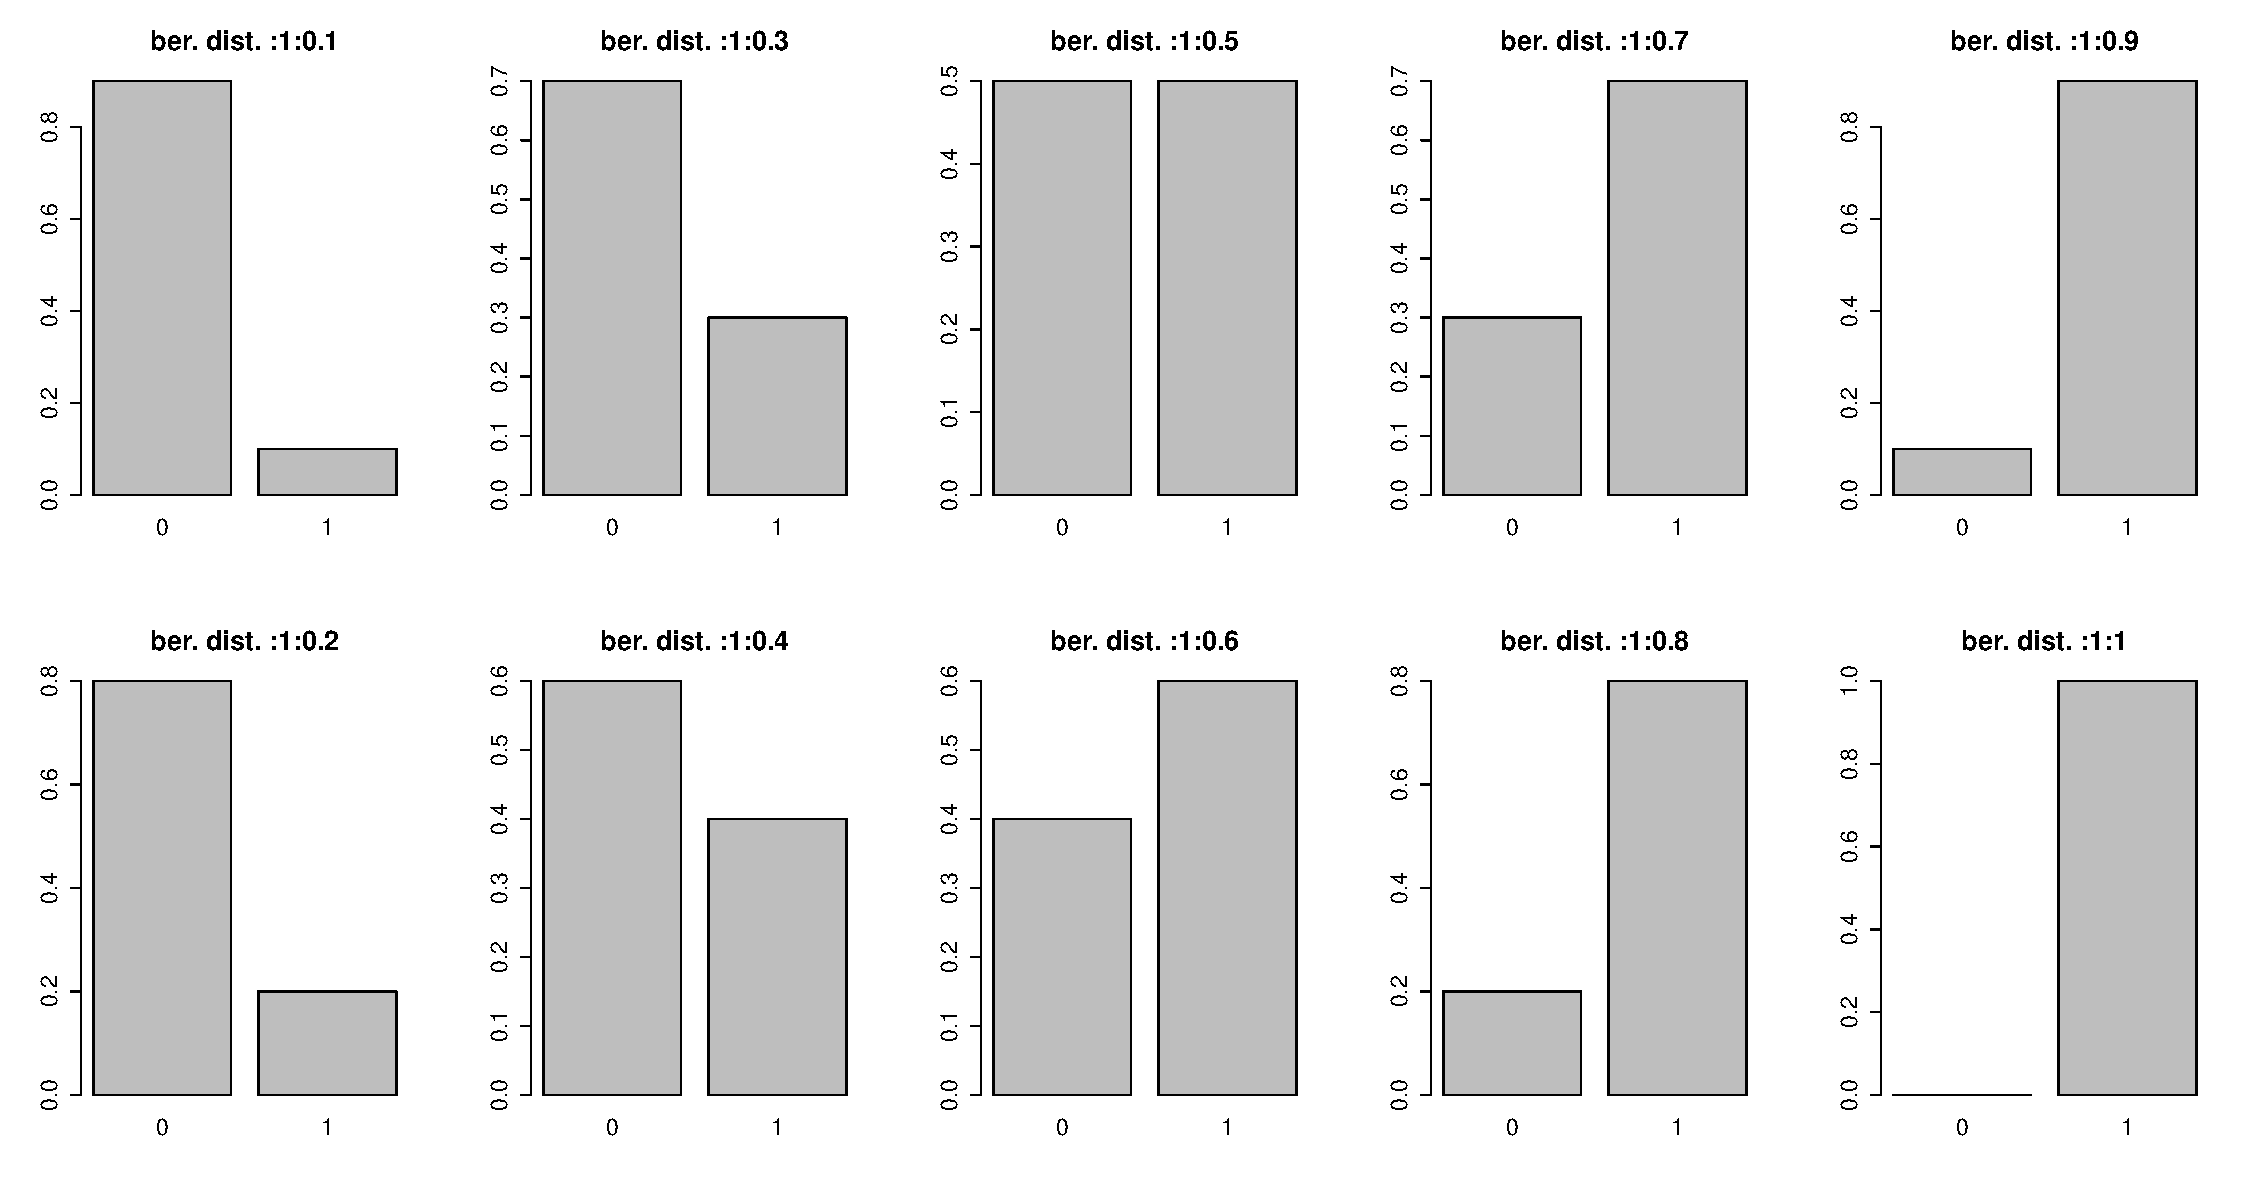
\includegraphics[width=10cm,keepaspectratio]{bernoulli_plots.pdf}

\end{frame}
%%%%%%%%%%%%%%%%%%%%%%%%%%%%%%%%%%%%%%%%%%%%%%%%%%%%%%%%%%%%

%%%%%%%%%%%%%%%%%%%%%%%%%%%%%%%%%%%%%%%%%%%%%%%%%%%%%%%%%%%%
\begin{frame}[fragile]{Binomial Distribution \;\;}
%%%%%%%%%%%%%%%%%%%%%%%%%%%%%%%%%%%%%%%%%%%%%%%%%%%%%%%%%%%%

Here $X$ denotes number of heads observed in $n$ tosses. Let probability of observing head in one toss be $p$

\begin{align}
Pr(X=0) & = (1-p)^{n} \\
Pr(X=1) & = np(1-p)^{n-1} \\
Pr(X=2) & = {n \choose k} p^2 (1-p)^{n-2} \\
....  &  ...  \\
Pr(X=x) & = {n \choose k} p^x (1-p)^{n-x}  \\
.... &  .... \\
Pr(X=n) & = p^{n} \\
\end{align}

$$ E(X) = ?  \hspace{0.5 cm} Var(X) = ?  $$

\end{frame}
%%%%%%%%%%%%%%%%%%%%%%%%%%%%%%%%%%%%%%%%%%%%%%%%%%%%%%%%%%%%

%%%%%%%%%%%%%%%%%%%%%%%%%%%%%%%%%%%%%%%%%%%%%%%%%%%%%%%%%%%%
\begin{frame}[fragile]{Binomial Distribution graph (n=20) \;\;}
%%%%%%%%%%%%%%%%%%%%%%%%%%%%%%%%%%%%%%%%%%%%%%%%%%%%%%%%%%%%


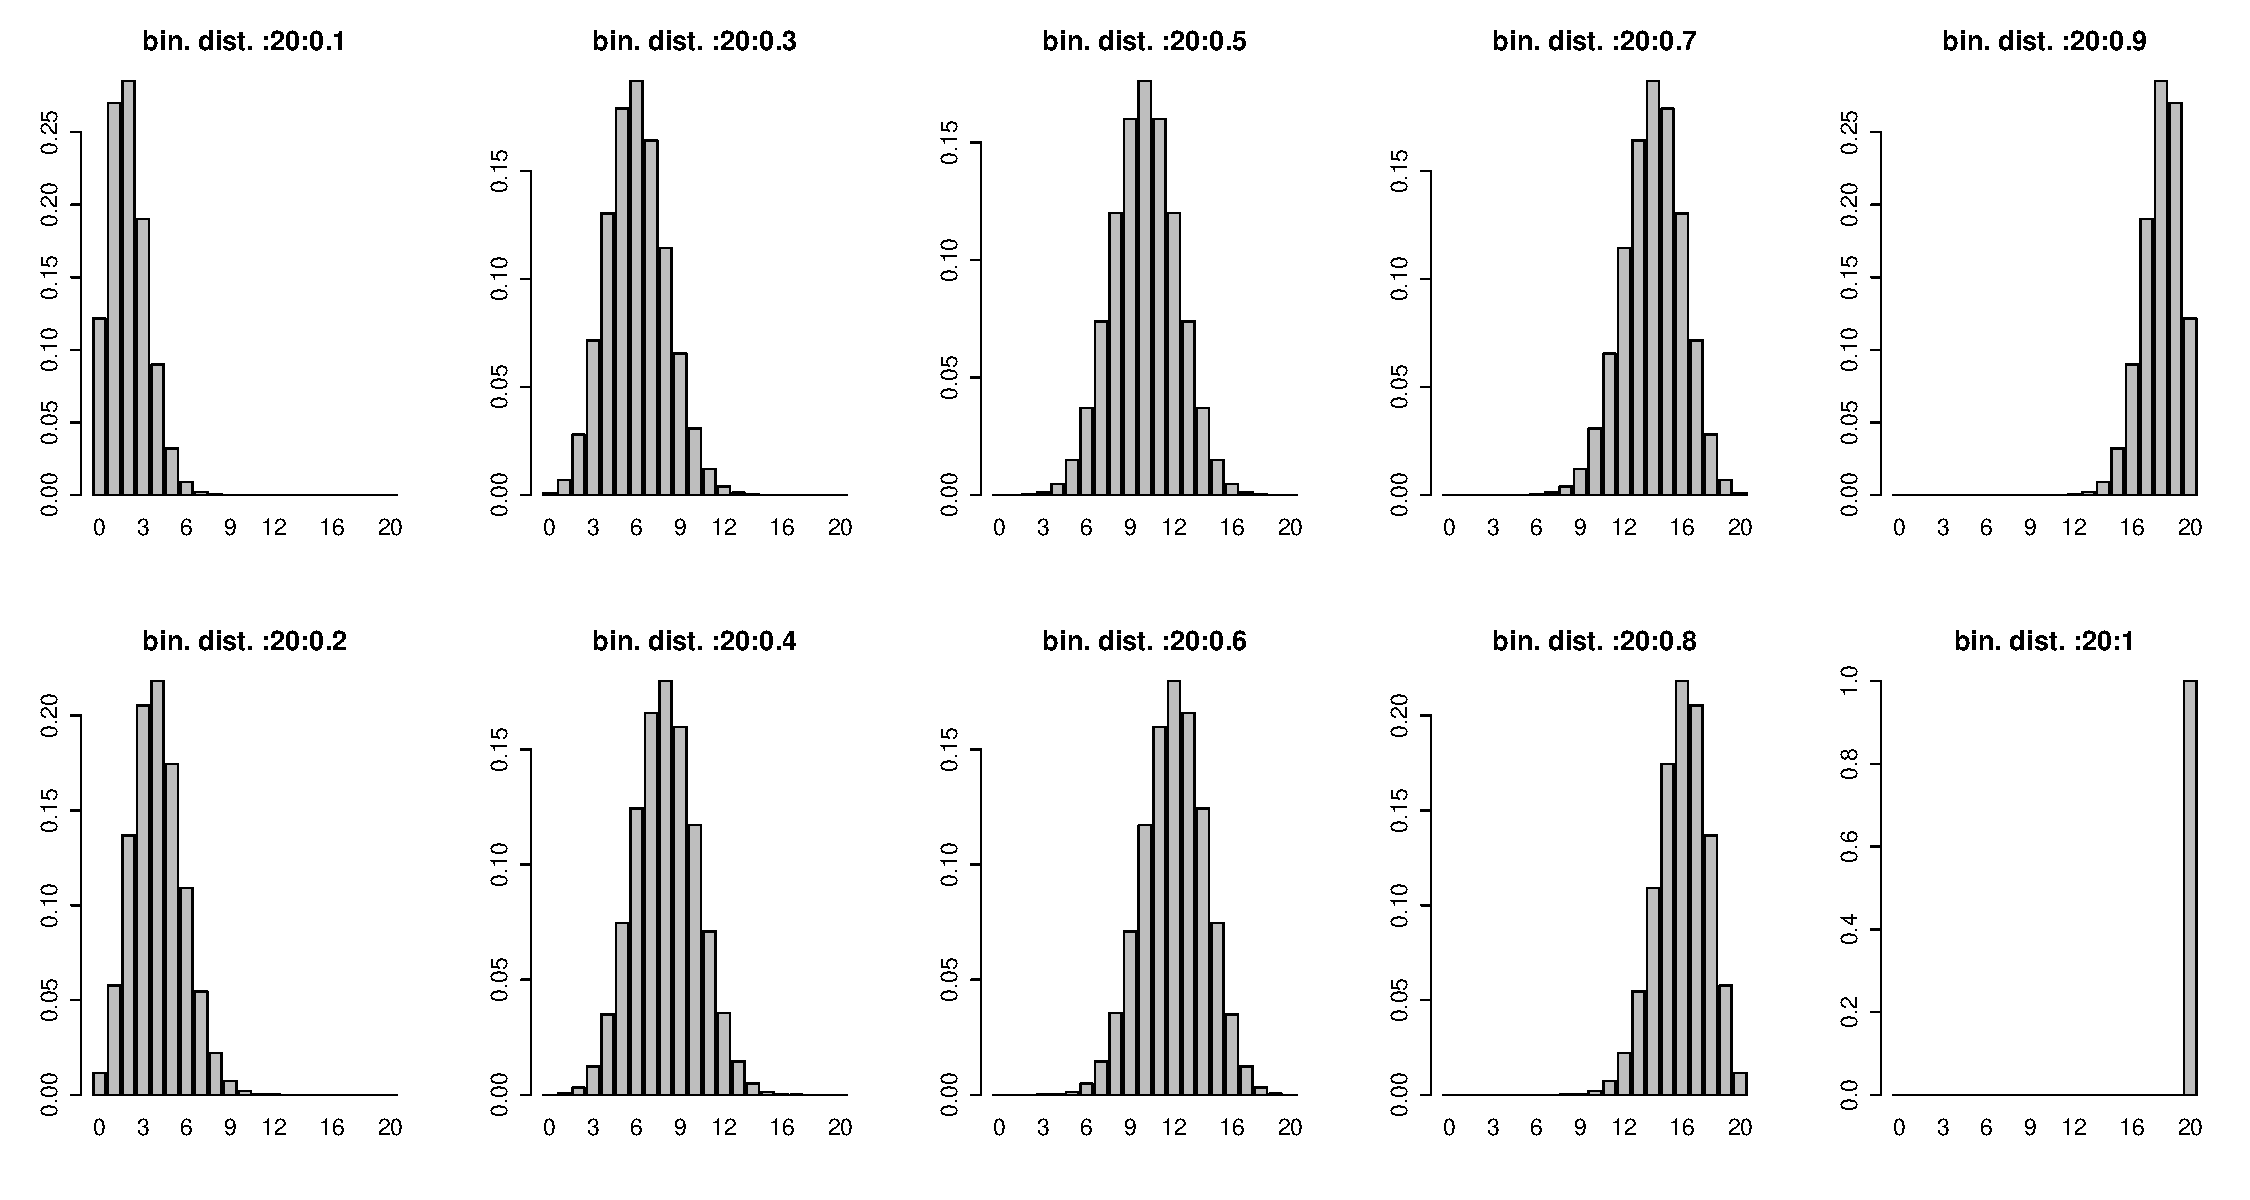
\includegraphics[width=10cm,keepaspectratio]{binomial_plots.pdf}
\end{frame}

%%%%%%%%%%%%%%%%%%%%%%%%%%%%%%%%%%%%%%%%%%%%%%%%%%%%%%%%%%%%
\begin{frame}[fragile]{Moment generating function \;\;}
%%%%%%%%%%%%%%%%%%%%%%%%%%%%%%%%%%%%%%%%%%%%%%%%%%%%%%%%%%%%

The moment generating function (mgf) is given by

\begin{align}
mgf(t) & : = E(e^{tX}) \\
& = E \left ( \left \{ \sum_{k=1}^{\infty} \frac{(tX)^{k}}{k!} \right \} Pr(X=k) \right) \\
& = \sum_{k=1}^{K} \frac{t^{k}}{k!} E \left ( X^{k} \right) \\
& = \sum_{k=1}^{K} \frac{t^{k}}{k!} \mu_{k}
\end{align}

$\mu_{k}$ is called the $k$th moment of the distribution of $X$. \pause \newline

Why do we care about $mgf(t)$?

\end{frame}
%%%%%%%%%%%%%%%%%%%%%%%%%%%%%%%%%%%%%%%%%%%%%%%%%%%%%%%%%%%%

%%%%%%%%%%%%%%%%%%%%%%%%%%%%%%%%%%%%%%%%%%%%%%%%%%%%%%%%%%%%
\begin{frame}[fragile]{The problem \;\;}
%%%%%%%%%%%%%%%%%%%%%%%%%%%%%%%%%%%%%%%%%%%%%%%%%%%%%%%%%%%%

\begin{center}
\Huge{Where is the connection to the last 4 classes?}
\end{center}

\end{frame}
%%%%%%%%%%%%%%%%%%%%%%%%%%%%%%%%%%%%%%%%%%%%%%%%%%%%%%%%%%%%


%%%%%%%%%%%%%%%%%%%%%%%%%%%%%%%%%%%%%%%%%%%%%%%%%%%%%%%%%%%%
\begin{frame}[fragile]{How to connect to previous classes \;\;}
%%%%%%%%%%%%%%%%%%%%%%%%%%%%%%%%%%%%%%%%%%%%%%%%%%%%%%%%%%%%

Suppose I want to find out what proportion of Males/Females study in UChicago. \pause \newline

I stand at the center of the Quad for a day and mark the gender of each person passing by. \pause \newline

Each record I take of a person is one run of the experiment. The states of the space
for one run is $\{ M, F \}$.

\end{frame}
%%%%%%%%%%%%%%%%%%%%%%%%%%%%%%%%%%%%%%%%%%%%%%%%%%%%%%%%%%%%


%%%%%%%%%%%%%%%%%%%%%%%%%%%%%%%%%%%%%%%%%%%%%%%%%%%%%%%%%%%%
\begin{frame}[fragile]{How to connect to previous classes \;\;}
%%%%%%%%%%%%%%%%%%%%%%%%%%%%%%%%%%%%%%%%%%%%%%%%%%%%%%%%%%%%

Say, if I observe $M$, I am noting down $1$ and if $F$, I am noting down $0$. \pause \newline

For the first record I note down, define

\begin{align}
X & = 1 \;\; if \;\; M \\
  & = 0 \;\; if \;\; F \\
\end{align}

$X$ is a random variable. \pause \newline

Assume the actual proportion of males in UChicago is $p$. We do not know $p$ (otherwise we would not have sampled). Then

$$  X \sim Ber(p)  $$ \pause \newline


\end{frame}
%%%%%%%%%%%%%%%%%%%%%%%%%%%%%%%%%%%%%%%%%%%%%%%%%%%%%%%%%%%%

%%%%%%%%%%%%%%%%%%%%%%%%%%%%%%%%%%%%%%%%%%%%%%%%%%%%%%%%%%%%
\begin{frame}[fragile]{How to connect to previous classes \;\;}
%%%%%%%%%%%%%%%%%%%%%%%%%%%%%%%%%%%%%%%%%%%%%%%%%%%%%%%%%%%%

Continue taking records. Suppose I have taken $100$ independent records.\pause \newline

My state space now is

$$ S = \left \{ (x_1 x_2 \cdots x_n) :  x_i \in \{ M, F \} \right \}  $$ \pause \newline

Now I can define $n$ random variables $X_1, X_2, \cdots, X_n$, so that

\begin{align}
X_1 & = 1 \;\; if \;\; (M x_2 x_3 \cdots x_n) \\
  & = 0 \;\; if \;\;  (F x_2 x_3 \cdots x_n) \\
\end{align}

and so on. \pause \newline

$$ X_{i} \stackrel{\sim}{iid} Ber (p)  $$ \pause \newline

We compute $Y= \sum_{i=1}^{n} X_{i}$

$$ Y \sim Bin(n,p) $$

\end{frame}
%%%%%%%%%%%%%%%%%%%%%%%%%%%%%%%%%%%%%%%%%%%%%%%%%%%%%%%%%%%%

%%%%%%%%%%%%%%%%%%%%%%%%%%%%%%%%%%%%%%%%%%%%%%%%%%%%%%%%%%%%
\begin{frame}[fragile]{How to connect to previous classes \;\;}
%%%%%%%%%%%%%%%%%%%%%%%%%%%%%%%%%%%%%%%%%%%%%%%%%%%%%%%%%%%%

Look at $ \frac{Y}{n} = \bar{X}_{n}$. Use that as an approximation for $p$. \pause \newline

The more sample records you choose, more is $n$ and by Law of Large numbers, the closer your approximation will be to the true value $p$. \pause \newline

In an ideal world, if you had managed to record all the students in Uchicago, you will be able to determine $p$ exactly. \pause \newline

The point of sampling is if by just recording $100/1000$ students can give you a somewhat close approximation to actual parameter $p$, why bother recording all students and waste your time and energy and resources? \pause \newline

\textbf{That is the main reason why we do Statistics!!}

\end{frame}
%%%%%%%%%%%%%%%%%%%%%%%%%%%%%%%%%%%%%%%%%%%%%%%%%%%%%%%%%%%%


%%%%%%%%%%%%%%%%%%%%%%%%%%%%%%%%%%%%%%%%%%%%%%%%%%%%%%%%%%%%
\begin{frame}[fragile]{A fun matching problem \;\;}
%%%%%%%%%%%%%%%%%%%%%%%%%%%%%%%%%%%%%%%%%%%%%%%%%%%%%%%%%%%%

\url{http://www.rossmanchance.com/applets/randomBabies/RandomBabies.html}

\end{frame}
%%%%%%%%%%%%%%%%%%%%%%%%%%%%%%%%%%%%%%%%%%%%%%%%%%%%%%%%%%%%

%%%%%%%%%%%%%%%%%%%%%%%%%%%%%%%%%%%%%%%%%%%%%%%%%%%%%%%%%%%%
\begin{frame}[fragile]{Joint Distribution \;\;}
%%%%%%%%%%%%%%%%%%%%%%%%%%%%%%%%%%%%%%%%%%%%%%%%%%%%%%%%%%%%

Consider two independent tosses of a coin. \newline

Let $X_1$ be the number of Ts observed in the 2 tosses. \newline

Let $X_2$ be $1$ if at least one $T$ observed, $0$ otherwise. \pause \newline

The table

\begin{tabular}{|c|c|c|c|}
\hline
states & $X_1$ & $X_2$ & Prob \\ \hline
HH & 0 & 0 & 0.25 \\ \hline
HT & 1 & 1 & 0.25 \\ \hline
TH & 1 & 1 & 0.25 \\ \hline
TT & 2 & 1 & 0.25 \\ \hline
\end{tabular}

\end{frame}
%%%%%%%%%%%%%%%%%%%%%%%%%%%%%%%%%%%%%%%%%%%%%%%%%%%%%%%%%%%%

%%%%%%%%%%%%%%%%%%%%%%%%%%%%%%%%%%%%%%%%%%%%%%%%%%%%%%%%%%%%
\begin{frame}[fragile]{Joint Probability Table \;\;}
%%%%%%%%%%%%%%%%%%%%%%%%%%%%%%%%%%%%%%%%%%%%%%%%%%%%%%%%%%%%

\begin{tabular}{|c|c|c|}
\hline
$X1|X2$ & 0 & 1 \\ \hline
0 & 0.25 & 0 \\ \hline
1 & 0 & 0.50 \\ \hline
2 & 0 & 0.25  \\ \hline
\end{tabular} \pause \newline \newline

\begin{tabular}{|c|c|c|c|}
\hline
$X1|X2$ & 0 & 1 & Total\\ \hline
0 & 0.25 & 0 & 0.25 \\ \hline
1 & 0 & 0.50 & 0.50\\ \hline
2 & 0 & 0.25 & 0.25\\ \hline
Total & 0.25 & 0.75 & 1 \\ \hline
\end{tabular}

\end{frame}
%%%%%%%%%%%%%%%%%%%%%%%%%%%%%%%%%%%%%%%%%%%%%%%%%%%%%%%%%%%%

%%%%%%%%%%%%%%%%%%%%%%%%%%%%%%%%%%%%%%%%%%%%%%%%%%%%%%%%%%%%
\begin{frame}[fragile]{Joint Probability Table \;\;}
%%%%%%%%%%%%%%%%%%%%%%%%%%%%%%%%%%%%%%%%%%%%%%%%%%%%%%%%%%%%

Marginal distribution of $X1$

\begin{tabular}{|c|c|c|c|}
$X1|X2$ & 0 & 1 & Total\\ \hline
0 & 0.25 & 0 & \textcolor{red}{0.25} \\ \hline
1 & 0 & 0.50 & \textcolor{red}{0.50}\\ \hline
2 & 0 & 0.25 & \textcolor{red}{0.25}\\ \hline
Total & 0.25 & 0.75 & \textcolor{red}{1} \\ \hline
\end{tabular} \pause \newline

Marginal distribution of $X2$ \pause \newline

\begin{tabular}{|c|c|c|c|}
\hline
$X1|X2$ & 0 & 1 & Total\\ \hline
0 & 0.25 & 0 & 0.25 \\ \hline
1 & 0 & 0.50 & 0.50\\ \hline
2 & 0 & 0.25 & 0.25\\ \hline
Total & \textcolor{red}{0.25} & \textcolor{red}{0.75} & \textcolor{red}{1} \\ \hline
\end{tabular}

\end{frame}
%%%%%%%%%%%%%%%%%%%%%%%%%%%%%%%%%%%%%%%%%%%%%%%%%%%%%%%%%%%%

%%%%%%%%%%%%%%%%%%%%%%%%%%%%%%%%%%%%%%%%%%%%%%%%%%%%%%%%%%%%
\begin{frame}[fragile]{Joint and Marginal Probabilities \;\;}
%%%%%%%%%%%%%%%%%%%%%%%%%%%%%%%%%%%%%%%%%%%%%%%%%%%%%%%%%%%%

For two random variables $X$ and $Y$, the joint probability

$$ p(x,y)  = Pr(X=x, Y=y) $$

where $x$ and $y$ are possible relaizations of the random variables $X$ and $Y$. \pause \newline

From what we observed in the last slide, marginal distribution of $X$

$$ p_X(x) = Pr(X=x) = \sum_{y} p(x,y) $$

where the $\sum_{y}$ is over all realizations of $Y$. \pause \newline

Similarly for $Y$

$$ p_Y(y) = Pr(Y=y) = \sum_{x} p(x,y) $$

\end{frame}
%%%%%%%%%%%%%%%%%%%%%%%%%%%%%%%%%%%%%%%%%%%%%%%%%%%%%%%%%%%%

%%%%%%%%%%%%%%%%%%%%%%%%%%%%%%%%%%%%%%%%%%%%%%%%%%%%%%%%%%%%
\begin{frame}[fragile]{Conditional Probabilities \;\;}
%%%%%%%%%%%%%%%%%%%%%%%%%%%%%%%%%%%%%%%%%%%%%%%%%%%%%%%%%%%%

we define a conditional probability as

$$ Pr(X=x | Y=y) = \frac{Pr(X=x, Y=y)}{Pr(Y=y)} = \frac{p_{XY}(x,y)}{p_{Y}(y)} $$

Intuition: Given we have observed realization $y$ of $Y$, what is the probability distribution of $X$. \pause \newline

The distribution of $X1$ conditional on $X2=0$ and $X2=1$ in the previous example. \pause \newline

\begin{tabular}{|c|c|c|c|}
\hline
$X1|X2$ & 0 & 1 \\ \hline
0 & 1 & 0  \\ \hline
1 & 0 & 0.67 \\ \hline
2 & 0 & 0.33 \\ \hline
Total & 1 & 1 \\ \hline
\end{tabular}

\end{frame}
%%%%%%%%%%%%%%%%%%%%%%%%%%%%%%%%%%%%%%%%%%%%%%%%%%%%%%%%%%%%

%%%%%%%%%%%%%%%%%%%%%%%%%%%%%%%%%%%%%%%%%%%%%%%%%%%%%%%%%%%%
\begin{frame}[fragile]{Conditional Probabilities \;\;}
%%%%%%%%%%%%%%%%%%%%%%%%%%%%%%%%%%%%%%%%%%%%%%%%%%%%%%%%%%%%

we define a conditional probability as

$$ Pr(X=x | Y=y) = \frac{Pr(X=x, Y=y)}{Pr(Y=y)} = \frac{p_{XY}(x,y)}{p_{Y}(y)} $$

Intuition: Given we have observed realization $y$ of $Y$, what is the probability distribution of $X$.

The distribution of $X2$ conditional on $X1=0$, $X1=1$ and $X1=2$ in the previous example. \pause \newline

\begin{tabular}{|c|c|c|c|}
\hline
$X1|X2$ & 0 & 1 & Total\\ \hline
0 & 1 & 0 & 1\\ \hline
1 & 0 & 1 & 1 \\ \hline
2 & 0 & 1 & 1  \\ \hline
\end{tabular}

\end{frame}
%%%%%%%%%%%%%%%%%%%%%%%%%%%%%%%%%%%%%%%%%%%%%%%%%%%%%%%%%%%%

%%%%%%%%%%%%%%%%%%%%%%%%%%%%%%%%%%%%%%%%%%%%%%%%%%%%%%%%%%%%
\begin{frame}[fragile]{Sum of random variables \;\;}
%%%%%%%%%%%%%%%%%%%%%%%%%%%%%%%%%%%%%%%%%%%%%%%%%%%%%%%%%%%%

Consider two independent tosses of a coin. \newline

Let $X_1$ be the number of Ts observed in the 2 tosses. \newline

Let $X_2$ be $1$ if at least one $T$ observed, $0$ otherwise. \pause \newline

The table

\begin{tabular}{|c|c|c|c|c|}
\hline
states & $X_1$ & $X_2$ & $Y=X_1+X_2$ & Prob \\ \hline
HH & 0 & 0 & 0 & 0.25 \\ \hline
HT & 1 & 1 & 2 & 0.25 \\ \hline
TH & 1 & 1 & 2 & 0.25 \\ \hline
TT & 2 & 1 & 3 & 0.25 \\ \hline
\end{tabular}

\end{frame}
%%%%%%%%%%%%%%%%%%%%%%%%%%%%%%%%%%%%%%%%%%%%%%%%%%%%%%%%%%%%

%%%%%%%%%%%%%%%%%%%%%%%%%%%%%%%%%%%%%%%%%%%%%%%%%%%%%%%%%%%%
\begin{frame}[fragile]{Sum of random variables \;\;}
%%%%%%%%%%%%%%%%%%%%%%%%%%%%%%%%%%%%%%%%%%%%%%%%%%%%%%%%%%%%

\begin{align}
E(Y) & = E(X_1 + X_2) \\
     & = 0 \times 0.25 + 2 \times 0.50 + 3 \times 0.25 \\
     & = 1.75 \\
\end{align} \pause

$$ E(X_1) = 1 \hspace{1 cm} E(X_2) = 0.75 $$ \pause

$$ E(X_1 + X_2) = E(X_1) + E(X_2)  $$ \pause

Is that always true? \pause YES!!! Lets derive it.

\end{frame}
%%%%%%%%%%%%%%%%%%%%%%%%%%%%%%%%%%%%%%%%%%%%%%%%%%%%%%%%%%%%

%%%%%%%%%%%%%%%%%%%%%%%%%%%%%%%%%%%%%%%%%%%%%%%%%%%%%%%%%%%%
\begin{frame}{Similar Results}
%%%%%%%%%%%%%%%%%%%%%%%%%%%%%%%%%%%%%%%%%%%%%%%%%%%%%%%%%%%%

\begin{itemize}

\item $E(c) = c $ where $c$ is constant
\item $E(aX) = a E(X)$
\item $ E(X+Y) = E(X) + E(Y) $
\item $ E(aX + bY) = a E(X) + b E(Y) $ where $a,b$ are constants.

\end{itemize}

\end{frame}
%%%%%%%%%%%%%%%%%%%%%%%%%%%%%%%%%%%%%%%%%%%%%%%%%%%%%%%%%%%%

%%%%%%%%%%%%%%%%%%%%%%%%%%%%%%%%%%%%%%%%%%%%%%%%%%%%%%%%%%%%
\begin{frame}{Expected Value of a Linear Combination}
%%%%%%%%%%%%%%%%%%%%%%%%%%%%%%%%%%%%%%%%%%%%%%%%%%%%%%%%%%%%

Show that $E(aX+bY) = aE(X) + bE(Y).$

\begin{align*}
&E(aX+bY) = \sum_x \sum_y
               (ax+by) p(x,y)\\
&\hid{2-}{=  \sum_x \sum_y ax p(x,y) + \sum_x \sum_y by p(x,y)}\\
&\hid{2-}{=  \sum_x \sum_y ax p(x,y) + \sum_y \sum_x by p(x,y)}\\
&\hid{3-}{= \sum_x ax
\underbrace{\left[\sum_y p(x,y)\right]}_{\hid{4-}{=p_X(x)}} + \sum_y by
\underbrace{\left[\sum_x p(x,y)\right]}_{\hid{5-}{=p_Y(y)}}\;\;*}\\
&\hid{6-}{= a \sum_x x p_X(x) + b \sum_y y  p_Y(y)}
\hskip2.5cm \hid{7-}{= aE(X) + bE(Y)}
\end{align*}
\hid{3-}{{\small{*\; See HW0 for more details about the ``double sum."}}}

\end{frame}
%%%%%%%%%%%%%%%%%%%%%%%%%%%%%%%%%%%%%%%%%%%%%%%%%%%%%%%%%%%%

%%%%%%%%%%%%%%%%%%%%%%%%%%%%%%%%%%%%%%%%%%%%%%%%%%%%%%%%%%%%
\begin{frame}{Independence of two random variables}
%%%%%%%%%%%%%%%%%%%%%%%%%%%%%%%%%%%%%%%%%%%%%%%%%%%%%%%%%%%%

\begin{itemize}
\item The variable  $X$ is {\bf independent} of variable $Y$ if its
chances are not affected by the variable $Y$,

$$ Pr[X=x | Y=y] = Pr[X=x]  \hspace{0.5 cm} \forall \; x \hspace{0.5 cm} each \;\; y$$

\item The following 3 definitions of independence are equivalent.
\begin{itemize}\normalsize
\item $Pr[X=x | Y=y] = Pr[X=x]$
\item $Pr[Y=y | X=x] = Pr[Y=y]$
\item $Pr[X=x, Y=y] = p_{XY}(x,y) = Pr[X=x]Pr[Y=y] = p_{X}(x)p_{Y}(y)$
\end{itemize}

\end{itemize}

\end{frame}
%%%%%%%%%%%%%%%%%%%%%%%%%%%%%%%%%%%%%%%%%%%%%%%%%%%%%%%%%%%%

%%%%%%%%%%%%%%%%%%%%%%%%%%%%%%%%%%%%%%%%%%%%%%%%%%%%%%%%%%%%
\begin{frame}{Independence for Random Variables}
%%%%%%%%%%%%%%%%%%%%%%%%%%%%%%%%%%%%%%%%%%%%%%%%%%%%%%%%%%%%
$$p(x,y) = p_X(x)p_Y(y).$$
Note: Independence implies that
$$p(y|X=x) = \frac{p(x,y)}{p_X(x)} = \frac{p_X(x)p_Y(y)}{p_X(x)} = p_Y(y).$$
\begin{center}
\begin{tabular}{l|c||c|c|c||c|}
\multicolumn{5}{c}{$X$}\\
\cline{2-6}
&&0&1&2&$p(y)$\\
\cline{2-6}
$Y$&0&2/6& 1/6&0&3/6\\
\cline{2-6}
   &1&0&1/6&2/6&3/6\\
\cline{2-6}
   &$p(x)$ &2/6&2/6&2/6&\\
\cline{2-6}
\end{tabular}
\end{center}

Consider the pair $(x,y,) = (0,0).$
$$p(0,0) = 2/6 \ne p_X(0)p_Y(0) = (1/3)(1/2) = 1/6.$$

$X$ and $Y$ are not independent.

\end{frame}
%%%%%%%%%%%%%%%%%%%%%%%%%%%%%%%%%%%%%%%%%%%%%%%%%%%%%%%%%%%%

%%%%%%%%%%%%%%%%%%%%%%%%%%%%%%%%%%%%%%%%%%%%%%%%%%%%%%%%%%%%
\begin{frame}{Covariance between Random Variables}
%%%%%%%%%%%%%%%%%%%%%%%%%%%%%%%%%%%%%%%%%%%%%%%%%%%%%%%%%%%%

The covariance between random variables $X$ and $Y$ is defined as

\begin{align}
cov(X,Y)  & = E(X- E(X)(Y-E(Y)))  \\
          &  = E(XY - E(X)Y - XE(Y) + E(X)E(Y)) \\
          &  = E(XY) - E(E(X)Y) - E(XE(Y)) + E(E(X)E(Y)) \\
          &  = E(XY) - E(X)E(Y) - E(X)E(Y) + E(X)E(Y) \\
          &  = E(XY) - E(X)E(Y) \\
          &  = \sum_{x,y} xy Pr(X=x, Y=y) - E(X)E(Y) \\
\end{align} \pause

When $X$ and $Y$ are independent, we also have $cov(X,Y)=0$ \pause \newline

The converse is not true!!
\end{frame}
%%%%%%%%%%%%%%%%%%%%%%%%%%%%%%%%%%%%%%%%%%%%%%%%%%%%%%%%%%%%

%%%%%%%%%%%%%%%%%%%%%%%%%%%%%%%%%%%%%%%%%%%%%%%%%%%%%%%%%%%%
\begin{frame}{Example to disprove the converse}
%%%%%%%%%%%%%%%%%%%%%%%%%%%%%%%%%%%%%%%%%%%%%%%%%%%%%%%%%%%%

Let $X$ be a random variable

\begin{align}
X & = 1 \;\; prob \;\; 0.5
  & = -1 \;\; prob \;\; 0.5
\end{align}

Let $Y$ be another random variable
\begin{align}
Y & = 0 \;\; if \; X=1 \\
  & = +1 \;\; if \; X=-1 \; prob \; 0.5 \\
  & = -1 \;\; if \; X=-1 \; prob \; 0.5 \\
 \end{align}

 Then check that $E(XY)=E(X)=E(Y)=0$ and so $cov(X,Y)=0$

 Show $X$ and $Y$ are not independent

 \end{frame}
%%%%%%%%%%%%%%%%%%%%%%%%%%%%%%%%%%%%%%%%%%%%%%%%%%%%%%%%%%%%

%%%%%%%%%%%%%%%%%%%%%%%%%%%%%%%%%%%%%%%%%%%%%%%%%%%%%%%%%%%%
\begin{frame}{Correlation between Random Variables}
%%%%%%%%%%%%%%%%%%%%%%%%%%%%%%%%%%%%%%%%%%%%%%%%%%%%%%%%%%%%

Correlation between two random variables $X$ and $Y$ is given by

$$ cor(X,Y) = \frac{cov(X,Y)}{\sqrt{var(X)}\sqrt{var(Y)}} $$

It can be shown that  (check Cauchy Schwartz inequality)

$$ -1 \leq cor(X,Y) \leq +1 $$

Correlation (and covariance) is a measure of \emph{linear} dependency.

Correaltion of $-1$ means negative linear dependency, $+1$ means positive linear dependency, $0$ means no linear dependency.

\end{frame}
%%%%%%%%%%%%%%%%%%%%%%%%%%%%%%%%%%%%%%%%%%%%%%%%%%%%%%%%%%%%

%%%%%%%%%%%%%%%%%%%%%%%%%%%%%%%%%%%%%%%%%%%%%%%%%%%%%%%%%%%%
\begin{frame}{Recap}
%%%%%%%%%%%%%%%%%%%%%%%%%%%%%%%%%%%%%%%%%%%%%%%%%%%%%%%%%%%%

- States of an experiment, Events, Random Variables

- Probability (Joint, Marginal and Conditional)

- Expectation, Variance, Moments, MGF

- Law of Large Numbers, Chebyshev Inequality

- Independence and Covariance

- Sums of random variables

- Connect with Statistical Data !!

\end{frame}
%%%%%%%%%%%%%%%%%%%%%%%%%%%%%%%%%%%%%%%%%%%%%%%%%%%%%%%%%%%%

%%%%%%%%%%%%%%%%%%%%%%%%%%%%%%%%%%%%%%%%%%%%%%%%%%%%%%%%%%%%
\begin{frame}{}
%%%%%%%%%%%%%%%%%%%%%%%%%%%%%%%%%%%%%%%%%%%%%%%%%%%%%%%%%%%%

\begin{center}
\Huge{Is there something I very conveniently skipped?}
\end{center}

\end{frame}
%%%%%%%%%%%%%%%%%%%%%%%%%%%%%%%%%%%%%%%%%%%%%%%%%%%%%%%%%%%%


%%%%%%%%%%%%%%%%%%%%%%%%%%%%%%%%%%%%%%%%%%%%%%%%%%%%%%%%%%%%
\begin{frame}{Continuous Random Variables}
%%%%%%%%%%%%%%%%%%%%%%%%%%%%%%%%%%%%%%%%%%%%%%%%%%%%%%%%%%%%

Position yourself again at the middle of the Quad. Suppose now you record the height of each person crossing the Quad. \pause \newline

In this case each person whose height is measured is a run of the experiment. The state is the height (in ft/inches). Since the state itself is numeric, we can directly define a random variable $X$ same as the state. \pause \newline

Now we record the states for $n$ individuals. Then the state space

$$ S = \left \{ (h_1 h_2 \cdots h_n) \right \} $$

and define $n$ random variables $X_1, X_2, \cdots, X_n$ such that

$$ X_1 = h_1 \hspace{0.5 cm} X_2=h_2 \hspace{0.5 cm}\cdots X_{n}=h_{n} $$

\end{frame}
%%%%%%%%%%%%%%%%%%%%%%%%%%%%%%%%%%%%%%%%%%%%%%%%%%%%%%%%%%%%

%%%%%%%%%%%%%%%%%%%%%%%%%%%%%%%%%%%%%%%%%%%%%%%%%%%%%%%%%%%%
\begin{frame}{Continuous Random Variables}
%%%%%%%%%%%%%%%%%%%%%%%%%%%%%%%%%%%%%%%%%%%%%%%%%%%%%%%%%%%%

If we had recorded the heights of all students, the assume the histogram would have been approximated by a normal bell-shaped curve with center $\mu$ and variance $\sigma^2$ very accurately.Then

$$ X_1, X_2, \cdots, X_{n} \stackrel{iid}{\sim} N(\mu, \sigma)  $$ \pause \newline

You can then build the histogram of the $n$ realizations. Then we fit a curve as a fit to the histogram. \pause \newline

\end{frame}
%%%%%%%%%%%%%%%%%%%%%%%%%%%%%%%%%%%%%%%%%%%%%%%%%%%%%%%%%%%%



%%%%%%%%%%%%%%%%%%%%%%%%%%%%%%%%%%%%%%%%%%%%%%%%%%%%%%%%%%%%
\begin{frame}{Continuous Random Variables}
%%%%%%%%%%%%%%%%%%%%%%%%%%%%%%%%%%%%%%%%%%%%%%%%%%%%%%%%%%%%

As $n \rightarrow \infty$, the fitted curve would get closer and closer to the normal bell-shaped curve with the above mean and variance parameters. \pause \newline

The sample mean $\bar{X}_{n}$ and sample standard deviation $s^2_{n}$ will also get closer and closer to $\mu$ and $\sigma$ respectively as $n \rightarrow \infty$. \pause \newline

But again, we save our time and energy by looking at only $100/1000$ samples and then approximate the normal model by approximately determining the population or model parameters $\mu$ and $\sigma$ from the $n$ data points and corresponding histogram.

\end{frame}
%%%%%%%%%%%%%%%%%%%%%%%%%%%%%%%%%%%%%%%%%%%%%%%%%%%%%%%%%%%%

%%%%%%%%%%%%%%%%%%%%%%%%%%%%%%%%%%%%%%%%%%%%%%%%%%%%%%%%%%%%
\begin{frame}{Continuous Probabilities}
%%%%%%%%%%%%%%%%%%%%%%%%%%%%%%%%%%%%%%%%%%%%%%%%%%%%%%%%%%%%

We would want to define $Pr(X=x)$ for a continuous random variable $X$, but unfortunately it is $0$. We will soon see why \pause \newline

So how do we proceed to build something like a probability table for discrete variable?

We define \textbf{cumulative density function} (cdf)

$$ F(x) = Pr (X \leq x) $$

If we differentiate this function, we get \textbf{probability density function} (pdf)

$$ \frac{d}{dx} F(x) = f(x) $$

$$ f(x) \geq 0 \hspace {1 cm} \int f(x) dx = 1 $$

\end{frame}
%%%%%%%%%%%%%%%%%%%%%%%%%%%%%%%%%%%%%%%%%%%%%%%%%%%%%%%%%%%%

%%%%%%%%%%%%%%%%%%%%%%%%%%%%%%%%%%%%%%%%%%%%%%%%%%%%%%%%%%%%
\begin{frame}{Continuous Probabilities}
%%%%%%%%%%%%%%%%%%%%%%%%%%%%%%%%%%%%%%%%%%%%%%%%%%%%%%%%%%%%

For normal distribution

$$ f(x)/ \phi(x) := \int \frac{1}{\sqrt{2 \pi}} exp \left (-\frac{(x-\mu)^2}{2 \sigma^2} \right ) $$

Cumulative distribution

$$ \Phi(x) : = \int_{-\infty}^{x} \phi(x) dx $$

Uniform distribution

$$ F(x) = Pr(X \leq x) = x $$

which implies $ f(x)=1$ for all $x$.

\end{frame}
%%%%%%%%%%%%%%%%%%%%%%%%%%%%%%%%%%%%%%%%%%%%%%%%%%%%%%%%%%%%


%%%%%%%%%%%%%%%%%%%%%%%%%%%%%%%%%%%%%%%%%%%%%%%%%%%%%%%%%%%%
\begin{frame}{cumulative density graphs (Uniform and Normal)}
%%%%%%%%%%%%%%%%%%%%%%%%%%%%%%%%%%%%%%%%%%%%%%%%%%%%%%%%%%%%

\begin{knitrout}\small
\definecolor{shadecolor}{rgb}{1, 1, 1}\color{fgcolor}

{\centering 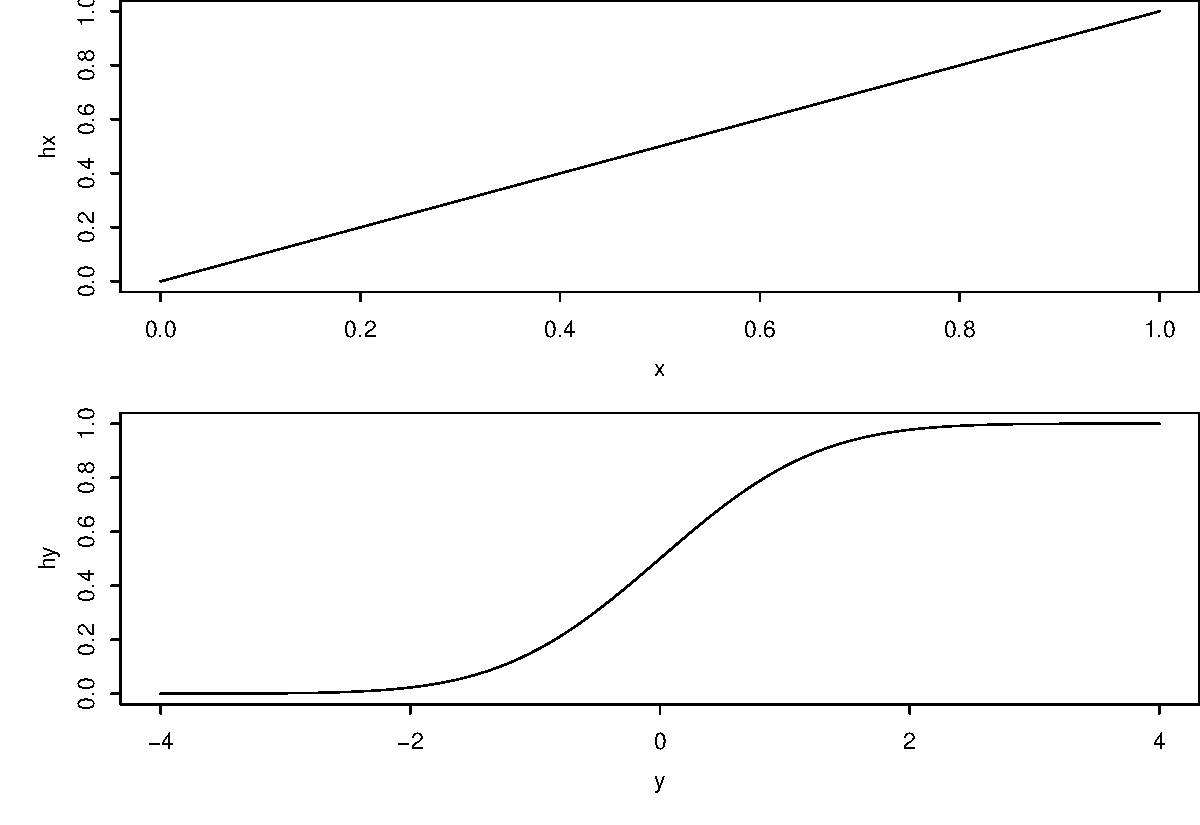
\includegraphics[width=0.99\linewidth]{figure/graphics-unnamed-chunk-4-1} 

}



\end{knitrout}

\end{frame}
%%%%%%%%%%%%%%%%%%%%%%%%%%%%%%%%%%%%%%%%%%%%%%%%%%%%%%%%%%%%

%%%%%%%%%%%%%%%%%%%%%%%%%%%%%%%%%%%%%%%%%%%%%%%%%%%%%%%%%%%%
\begin{frame}{probability density graphs (Uniform and Normal)}
%%%%%%%%%%%%%%%%%%%%%%%%%%%%%%%%%%%%%%%%%%%%%%%%%%%%%%%%%%%%

\begin{knitrout}\small
\definecolor{shadecolor}{rgb}{1, 1, 1}\color{fgcolor}

{\centering 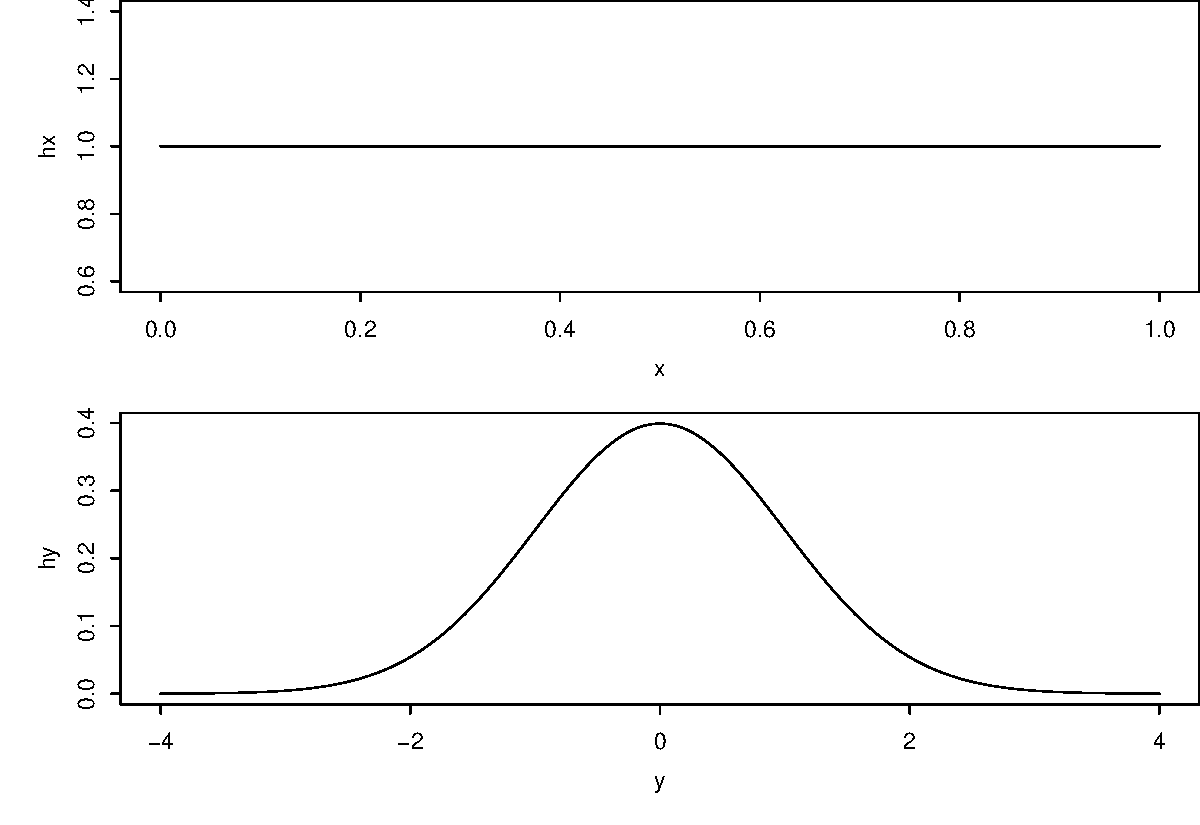
\includegraphics[width=0.99\linewidth]{figure/graphics-unnamed-chunk-5-1} 

}



\end{knitrout}

\end{frame}
%%%%%%%%%%%%%%%%%%%%%%%%%%%%%%%%%%%%%%%%%%%%%%%%%%%%%%%%%%%%

%%%%%%%%%%%%%%%%%%%%%%%%%%%%%%%%%%%%%%%%%%%%%%%%%%%%%%%%%%%%
\begin{frame}{Properties of Continous Random Variable}
%%%%%%%%%%%%%%%%%%%%%%%%%%%%%%%%%%%%%%%%%%%%%%%%%%%%%%%%%%%%

We define the expectation analogous to the discrete random variable.

$$ E(X): = \int x f(x) dx $$

$$ var(X) : = E(X-E(X))^2 = \int x^2 f(x) dx - E^2(X) $$

$$ MGF(t): = E(e^{tX}) = \int e^{tx} f(x) dx $$

For normal distribution, one can easily show that

$$ E(X) = \mu \hspace{0.5 cm} var(X)=\sigma^2 \hspace{0.5 cm} MGF(t) = exp(\mu t + \frac{\sigma^2t^2}{2}) $$

what about uniform? HW

\end{frame}
%%%%%%%%%%%%%%%%%%%%%%%%%%%%%%%%%%%%%%%%%%%%%%%%%%%%%%%%%%%%

%%%%%%%%%%%%%%%%%%%%%%%%%%%%%%%%%%%%%%%%%%%%%%%%%%%%%%%%%%%%
\begin{frame}{Properties of Continous Random Variable}
%%%%%%%%%%%%%%%%%%%%%%%%%%%%%%%%%%%%%%%%%%%%%%%%%%%%%%%%%%%%

For two continuous random variables $X$ and $Y$, we can define the joint cumulative density

$$ F(x,y) = Pr (X \leq x, Y \leq y) $$

Then we define joint density

$$ f(x,y) = \frac{d^2}{dxdy} F(x,y) = f_{XY}(x,y) $$

Define marginal

$$ \int_{X} f_{XY}(x,y) = f_{Y}(y) \hspace{0.5 cm} \int_{Y} f_{XY}(x,y) = f_{X}(x) $$

Conditional

$$ f_{X|Y}(x|y) : = \frac{f_{XY}(x,y)}{f_{Y}(y)}  $$

\end{frame}
%%%%%%%%%%%%%%%%%%%%%%%%%%%%%%%%%%%%%%%%%%%%%%%%%%%%%%%%%%%%

%%%%%%%%%%%%%%%%%%%%%%%%%%%%%%%%%%%%%%%%%%%%%%%%%%%%%%%%%%%%
\begin{frame}{Properties of Continous Random Variable}
%%%%%%%%%%%%%%%%%%%%%%%%%%%%%%%%%%%%%%%%%%%%%%%%%%%%%%%%%%%%

We say $X$ and $Y$ are independent when

$$ f_{X|Y}(x|y) = f_{X}(x)  $$

or

$$ f_{XY}(x,y)=f_{X}(x)f_{Y}(y) $$

As for discrete variables, independence implies uncorrelated but converse
is not true.

Similarly results related to sums and linear transform of two or more variables
stay true even for continuous variables.

\end{frame}
%%%%%%%%%%%%%%%%%%%%%%%%%%%%%%%%%%%%%%%%%%%%%%%%%%%%%%%%%%%%





\end{document}








